\documentclass{article}
\usepackage[UTF8]{ctex} 
\usepackage{amsmath}
\usepackage{bm}
\usepackage{amssymb}
\usepackage{geometry}
\usepackage{graphicx}
\usepackage{listings}
\usepackage{tikz}
\usepackage{amsthm}
\usetikzlibrary{shapes.multipart}
\usetikzlibrary{arrows.meta, positioning, shapes.geometric}
\usetikzlibrary{decorations.pathreplacing, fit}
\geometry{a4paper, margin=1.5cm}

\title{图(3)}
\author{Tan Yiqing}
\date{\today}

\begin{document}
\maketitle
    
    \begin{figure}[h]
        \centering
        \includegraphics[width=0.6\textwidth]{D:/program/data_construction/firefly/_20251124172156_504_13.jpg}
    \end{figure}

\section{最小生成树}
\subsection{基本概念}
\begin{enumerate}
    \item 生成树:n个顶点的连通图G的生成树是包含G中全部顶点的一个极小连通子图。(恰好含有n-1条边的连通图)
    \item 生成森林:在非连通图中,由每个连通分量都可以得到一棵生成树,
    这些连通分量的生成树就组成了一个非连通图的生成森林。
    \item 生成树的代价:设G = (V, E)是一个无向连通网,生成树上各边的权值之和称为该生成树的代价。
    \item 最小生成树:在图G所有生成树中,代价最小的生成树称为最小生成树。
\end{enumerate}

\subsection{最小生成树的性质}
\indent 最小生成树(MST)的性质:假设$G=(V, E)$是一个无向连通网,U是顶点集V的一个非空子集。若$(u, v)$是一条具有最小权值的边,其中$u\in U$,$v\in V-U$,则必存在一棵包含边$(u, v)$的最小生成树。\\
\indent 人话:在无向连通网 (G=(V,E)) 中,随便取一个非空真子集$ (U \subset V)$(比如把点分成“左边一堆”和“右边一堆”)。
看所有一端在 (U)、另一端在 (V-U) 的边(也就是“跨过这条分界线”的边)里,
如果 ((u,v)) 是其中权值最小的一条$(u\in U, v\in V-U)$,
那么:一定存在一棵最小生成树,包含这条边 ((u,v))。

\begin{figure}[h]
    \centering
    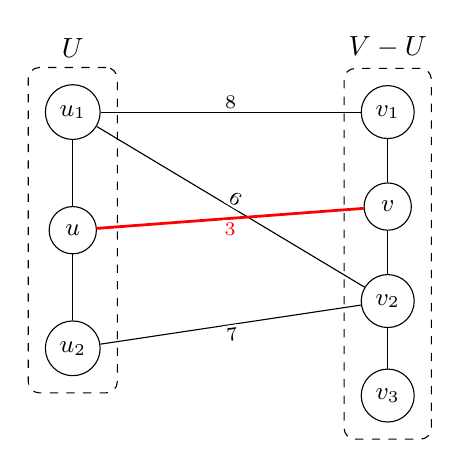
\begin{tikzpicture}[
        >=Stealth,
        node distance=14mm,
        v/.style={circle, draw, minimum size=6mm, font=\small},
        e/.style={-},
        cut/.style={-latex, dashed, gray},
        best/.style={line width=1pt, red},
        lbl/.style={font=\scriptsize, fill=white, inner sep=1pt}
    ]
        % 左侧 U
        \node[v] (u1) at (0,1.5) {$u_1$};
        \node[v] (u2) at (0,0)   {$u$};
        \node[v] (u3) at (0,-1.5){$u_2$};

        % 右侧 V-U
        \node[v] (v1) at (4,1.5) {$v_1$};
        \node[v] (v2) at (4,0.3) {$v$};
        \node[v] (v3) at (4,-0.9){$v_2$};
        \node[v] (v4) at (4,-2.1){$v_3$};

        % U 内部若干边
        \draw[e] (u1) -- (u2);
        \draw[e] (u2) -- (u3);

        % V-U 内部若干边
        \draw[e] (v1) -- (v2);
        \draw[e] (v2) -- (v3);
        \draw[e] (v3) -- (v4);

        % 割(U, V-U)之间的边(普通)
        \draw[e] (u1) -- (v1) node[pos=.5, above, lbl]{8};
        \draw[e] (u1) -- (v3) node[pos=.5, above, sloped, lbl]{6};
        \draw[e] (u3) -- (v3) node[pos=.5, below, sloped, lbl]{7};

        % 权值最小的边 (u, v),用红色粗线标出
        \draw[best] (u2) -- (v2) node[pos=.5, below, lbl]{3};

        % 画出割集虚线框,标出 U 与 V-U
        \node[draw, dashed, rounded corners, fit=(u1)(u2)(u3),
              inner sep=6pt, label=above:$U$] (Ubox) {};
        \node[draw, dashed, rounded corners, fit=(v1)(v2)(v3)(v4),
              inner sep=6pt, label=above:$V-U$] (Vbox) {};

    \end{tikzpicture}
    \caption{跨割$(U, V-U)$的最小权边$(u,v)$必在某棵最小生成树中}
\end{figure}



\subsection{Prim算法}
\subsubsection{算法思想}
\indent Prim 算法是一种构造\pmb{最小生成树}的贪心算法。基本思想是:从图中任意一个顶点 $v_0$ 出发,把 $v_0$ 视为当前生成树的唯一顶点集合 $U=\{v_0\}$,生成树边集合 $TE=\varnothing$。在每一步中,从所有一端在 $U$、另一端在 $V-U$ 的边中,选取权值最小的边 $(u,v)$,将顶点 $v$ 加入 $U$,并把边 $(u,v)$ 加入 $TE$。重复这一过程,直到 $U=V$,即所有顶点都被纳入生成树,此时 $(V,TE)$ 就是一棵最小生成树。\\
\indent 之所以该算法正确,是因为利用了最小生成树的上述\pmb{性质}:对于任意非空真子集 $U\subset V$,所有跨越割 $(U,V-U)$ 的边中,权值最小的那条边必然属于某棵最小生成树。

\subsubsection{算法步骤}
\indent 设 $G=(V,E)$ 是一个有 $n$ 个顶点的无向连通网,顶点编号为 $1,2,\dots,n$。以顶点 $1$ 为起点构造最小生成树。使用集合和边集表示的伪代码如下:
\begin{enumerate}
    \item 初始化:
    \[
        U=\{1\},\qquad TE=\varnothing.
    \]
    \item 重复下述操作直到 $U=V$:
    \begin{enumerate}
        \item 在边集 $E$ 中寻找一条权值最小的边 $(u,v)$,满足
        \[
            u\in U,\qquad v\in V-U.
        \]
        \item 扩展顶点集合:
        \[
            U \leftarrow U\cup\{v\}.
        \]
        \item 扩展生成树边集合:
        \[
            TE \leftarrow TE\cup\{(u,v)\}.
        \]
    \end{enumerate}
    \item 当 $U=V$ 时算法结束,边集 $TE$ 中恰有 $n-1$ 条边,$(V,TE)$ 为一棵最小生成树。
\end{enumerate}

\noindent 实际实现时,为了快速找到当前满足 $u\in U, v\in V-U$ 且权值最小的边 $(u,v)$,通常会引入两个辅助数组:
\begin{itemize}
    \item $dist[i]$:表示当前从集合 $U$ 到顶点 $i$ 的\pmb{最小边权}(若 $i\in U$,可置为 $0$ 或 $+\infty$);
    \item $path[i]$:当 $i\notin U$ 时,$path[i]$ 是与 $i$ 相连、且属于 $U$ 的顶点的编号,使得边 $(path[i],i)$ 的权值等于 $dist[i]$。
\end{itemize}

\subsubsection{举例分析}
\indent 考虑如下无向连通网 $G=(V,E)$,其中
\[
V=\{1,2,3,4,5\},
\]
边及其权值如下(无向图中只写一次):\\
$(1,2,2)$,$(1,3,6)$,$(1,4,5)$,$(2,3,3)$,$(2,5,4)$,$(3,4,1)$,$(3,5,8)$,$(4,5,7)$。

\begin{figure}[h]
    \centering
    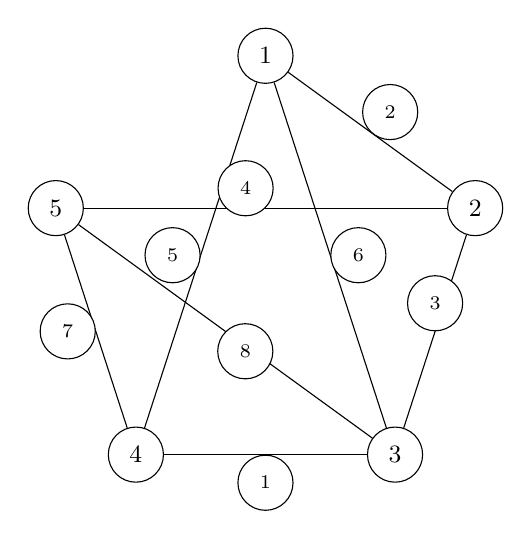
\begin{tikzpicture}[
        >=Stealth,
        every node/.style={circle, draw, minimum size=7mm, font=\small},
        edge/.style={-},
        w/.style={font=\scriptsize, fill=white, inner sep=1pt}
    ]
        % 正五边形布点
        \def\r{2.8}
        \path
            (90:\r)   node (v1) {$1$}
            (18:\r)   node (v2) {$2$}
            (306:\r)  node (v3) {$3$}
            (234:\r)  node (v4) {$4$}
            (162:\r)  node (v5) {$5$};

        % 无向边(画成直线)
        \draw[edge] (v1) -- (v2) node[midway, above right, w]{2};
        \draw[edge] (v1) -- (v3) node[midway, right, w]{6};
        \draw[edge] (v1) -- (v4) node[midway, left, w]{5};
        \draw[edge] (v2) -- (v3) node[midway, above, w]{3};
        \draw[edge] (v2) -- (v5) node[midway, above left, w]{4};
        \draw[edge] (v3) -- (v4) node[midway, below, w]{1};
        \draw[edge] (v3) -- (v5) node[midway, below right, w]{8};
        \draw[edge] (v4) -- (v5) node[midway, left, w]{7};
    \end{tikzpicture}
    \caption{Prim 算法示例图(无向连通网)}
\end{figure}

\noindent 以顶点 $1$ 为起点:

\begin{itemize}
    \item \textbf{初始化}:\\
    $U=\{1\}$,$TE=\varnothing$。
    \item \textbf{第 1 步}:
    \begin{enumerate}
        \item 在所有满足 $u\in U=\{1\}$、$v\in V-U=\{2,3,4,5\}$ 的边里:
        \[
            (1,2,2),\ (1,3,6),\ (1,4,5)
        \]
        其中权值最小的是 $(1,2,2)$。
        \item 令 $U=U\cup\{2\}=\{1,2\}$。
        \item 令 $TE=TE\cup\{(1,2)\}=\{(1,2)\}$。
    \end{enumerate}

    \item \textbf{第 2 步}:
    \begin{enumerate}
        \item 此时 $U=\{1,2\}$,$V-U=\{3,4,5\}$。所有跨越割 $(U,V-U)$ 的边有:
        \[
            (1,3,6),\ (1,4,5),\ (2,3,3),\ (2,5,4),
        \]
        其中权值最小的是 $(2,3,3)$。
        \item 令 $U=\{1,2,3\}$。
        \item 令 $TE=\{(1,2),(2,3)\}$。
    \end{enumerate}

    \item \textbf{第 3 步}:
    \begin{enumerate}
        \item 现在 $U=\{1,2,3\}$,$V-U=\{4,5\}$。跨越割的边有:
        \[
            (1,4,5),\ (2,5,4),\ (3,4,1),\ (3,5,8),
        \]
        其中权值最小的是 $(3,4,1)$。
        \item 令 $U=\{1,2,3,4\}$。
        \item 令 $TE=\{(1,2),(2,3),(3,4)\}$。
    \end{enumerate}

    \item \textbf{第 4 步}:
    \begin{enumerate}
        \item 此时 $U=\{1,2,3,4\}$,$V-U=\{5\}$。跨越割的边有:
        \[
            (2,5,4),\ (3,5,8),\ (4,5,7),
        \]
        最小的是 $(2,5,4)$。
        \item 令 $U=\{1,2,3,4,5\}=V$。
        \item 令 $TE=\{(1,2),(2,3),(3,4),(2,5)\}$。
    \end{enumerate}
\end{itemize}

\noindent 由于此时 $U=V$,算法结束。得到的一棵最小生成树为:
\[
TE=\{(1,2),\ (2,3),\ (3,4),\ (2,5)\},
\]
其代价为
\[
w(1,2)+w(2,3)+w(3,4)+w(2,5)=2+3+1+4=10.
\]



\subsection{Kruskal算法}
\subsubsection{算法思想}
\indent Kruskal 算法同样是构造\pmb{最小生成树}的贪心算法,但它不是“从一个点开始往外扩展”,而是“从所有边里由小到大挑,不断把连通分量合并”。\\
\indent 设无向连通网为 $G=(V,E)$,令 $G$ 的最小生成树为 $T=(U,TE)$。初始时 $U=V$(每个顶点单独看作一个连通分量),$TE=\varnothing$(还没有边)。然后按照边的权值由小到大依次考察 $E$ 中的各条边,对每条被考察的边:
\begin{itemize}
    \item 若该边的两个端点属于 $T$ 中\pmb{不同}的连通分量,则将此边加入 $TE$,并把这两个连通分量合并成一个;
    \item 若该边的两个端点已经在 $T$ 中的\pmb{同一个}连通分量,则舍去此边,以免在生成树中产生回路。
\end{itemize}
\indent 按此过程继续下去,当 $T$ 中只剩下一个连通分量(即 $TE$ 中已有 $|V|-1$ 条边)时,这个连通分量就是 $G$ 的一棵最小生成树。

\subsubsection{算法步骤}
\indent 设 $G=(V,E)$ 为无向连通网,$|V|=n$。用「并查集」或等价的“连通分量编号”来判断两个顶点是否在同一连通分量中。记每个连通分量的代表为 $Find(v)$。
\begin{enumerate}
    \item 初始化:
    \begin{enumerate}
        \item $U\leftarrow V$,$TE\leftarrow\varnothing$;
        \item 对每个顶点 $v\in V$,单独作为一个连通分量,$parent[v]\leftarrow v$(并查集初始化)。
    \end{enumerate}
    \item 将边集 $E$ 中的所有边按权值从小到大排序,得到有序序列
    \[
        (u_1,v_1,w_1), (u_2,v_2,w_2), \dots, (u_m,v_m,w_m),
        \quad w_1\le w_2\le\dots\le w_m.
    \]
    \item 依次扫描排好序的各条边,直至 $TE$ 中已有 $n-1$ 条边:
    \begin{enumerate}
        \item 取当前被考察的边 $(u_k,v_k,w_k)$;
        \item 若 $Find(u_k)\neq Find(v_k)$($u_k$ 与 $v_k$ 不在同一连通分量):
        \begin{itemize}
            \item 将此边加入生成树边集:
            \[
                TE \leftarrow TE\cup\{(u_k,v_k)\};
            \]
            \item 用合并操作将这两个连通分量合并:
            \[
                Union(Find(u_k), Find(v_k)).
            \]
        \end{itemize}
        \item 否则($Find(u_k)=Find(v_k)$,已在同一连通分量),舍去此边,继续考察下一条。
    \end{enumerate}
    \item 当 $|TE|=n-1$ 时,算法结束。此时 $(V,TE)$ 为一棵最小生成树。
\end{enumerate}

\subsubsection{举例分析}
\indent 使用与 Prim 算法相同的无向连通网 $G=(V,E)$:
\[
V=\{1,2,3,4,5\},
\]
边及其权值(无向边只写一次)为:
\[
(1,2,2),\ (1,3,6),\ (1,4,5),\ (2,3,3),\ (2,5,4),\ (3,4,1),\ (3,5,8),\ (4,5,7).
\]
其示意图如图 \ref{fig:prim-graph} 所示(与 Prim 示例图相同)。

\begin{figure}[h]
    \centering
    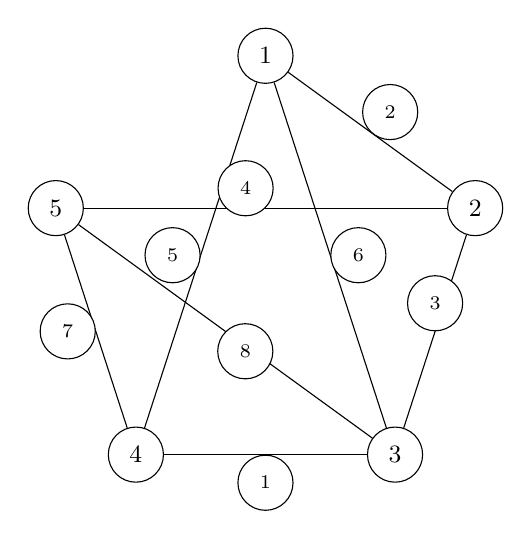
\begin{tikzpicture}[
        >=Stealth,
        every node/.style={circle, draw, minimum size=7mm, font=\small},
        edge/.style={-},
        w/.style={font=\scriptsize, fill=white, inner sep=1pt}
    ]
        \def\r{2.8}
        \path
            (90:\r)   node (v1) {$1$}
            (18:\r)   node (v2) {$2$}
            (306:\r)  node (v3) {$3$}
            (234:\r)  node (v4) {$4$}
            (162:\r)  node (v5) {$5$};

        \draw[edge] (v1) -- (v2) node[midway, above right, w]{2};
        \draw[edge] (v1) -- (v3) node[midway, right, w]{6};
        \draw[edge] (v1) -- (v4) node[midway, left, w]{5};
        \draw[edge] (v2) -- (v3) node[midway, above, w]{3};
        \draw[edge] (v2) -- (v5) node[midway, above left, w]{4};
        \draw[edge] (v3) -- (v4) node[midway, below, w]{1};
        \draw[edge] (v3) -- (v5) node[midway, below right, w]{8};
        \draw[edge] (v4) -- (v5) node[midway, left, w]{7};
    \end{tikzpicture}
    \caption{Kruskal 算法示例图(与 Prim 示例图相同)}
    \label{fig:prim-graph}
\end{figure}

\noindent 按照 Kruskal 算法的“边排序+连通分量合并”的思路进行:

\paragraph{1. 边按权值排序}
将所有边按权值从小到大排序:
\[
(3,4,1),\ (1,2,2),\ (2,3,3),\ (2,5,4),\ (1,4,5),\ (1,3,6),\ (4,5,7),\ (3,5,8).
\]
初始时,每个顶点自成一个连通分量:
\[
\{1\},\ \{2\},\ \{3\},\ \{4\},\ \{5\},\quad TE=\varnothing.
\]

\paragraph{2. 按顺序依次考察每条边}
\begin{itemize}
    \item 考察 $(3,4,1)$:$3$ 与 $4$ 在不同分量 $\{3\}$、$\{4\}$ 中,加入:
    \[
        TE=\{(3,4)\},\quad \text{分量:}\{1\},\{2\},\{3,4\},\{5\}.
    \]
    \item 考察 $(1,2,2)$:$1$ 与 $2$ 在不同分量 $\{1\}$、$\{2\}$ 中,加入:
    \[
        TE=\{(3,4),(1,2)\},\quad \text{分量:}\{1,2\},\{3,4\},\{5\}.
    \]
    \item 考察 $(2,3,3)$:$2$ 属于分量 $\{1,2\}$,$3$ 属于分量 $\{3,4\}$,不同分量,加入:
    \[
        TE=\{(3,4),(1,2),(2,3)\},\quad \text{分量:}\{1,2,3,4\},\{5\}.
    \]
    \item 考察 $(2,5,4)$:$2$ 属于分量 $\{1,2,3,4\}$,$5$ 属于分量 $\{5\}$,不同分量,加入:
    \[
        TE=\{(3,4),(1,2),(2,3),(2,5)\},\quad \text{分量:}\{1,2,3,4,5\}.
    \]
\end{itemize}

此时 $TE$ 中已经有 $|V|-1=4$ 条边,所有顶点被连接成一个连通分量,算法结束,后面的边 $(1,4,5)$、$(1,3,6)$、$(4,5,7)$、$(3,5,8)$ 即使再看也不会加入 MST(它们都会在已有的同一连通分量内形成回路)。\\

\noindent 最终得到的一棵最小生成树为:
\[
TE=\{(3,4),\ (1,2),\ (2,3),\ (2,5)\},
\]
其总代价为
\[
1+2+3+4=10.
\]

\subsubsection{Kruskal算法的数据结构设计}
\indent 该算法的难点在于如何判别被考察边的两个顶点是否位于两个连通分量。 \\
\indent Kruskal算法实质上是使生成树以一种随意的方式生长,初始时每个顶点构成一棵生成树,然后每生长一次就将两棵树合并,到最后合并成一棵树。

\indent 因此,可以设置一个数组parent[n],元素parent[i]表示顶点i的双亲结点,
初始时,parent[i]= -1,表示顶点i没有双亲,即该结点是所在生成树的根结点;
对于边(u, v),设vex1和vex2分别表示两个顶点所在树的根结点,如果vex1≠vex2,则顶点u和v必位于不同的连通分量,令parent[vex2] = vex1,实现将两棵树合并。
求某顶点v所在生成树的根结点只需沿数组v = parent[v]不断查找v的双亲,直到parent[v]等于-1。

\subsection{(了解)Reverse Delete Algorithm}
\indent Reverse Delete Algorithm(反向删除算法)也是一种用于寻找最小生成树的贪心算法。
其基本思想是从图的所有边开始,按权值从大到小排序,然后依次考虑每条边,判断是否可以删除该边而不破坏图的连通性。
如果删除该边后图仍然连通,则将该边删除;否则保留该边。最终剩下的边构成的子图即为最小生成树。

\section{有向无环图(DAG)}
\subsection{AOV网}
\subsubsection{基本概念}
\indent \pmb{AOV网(Activity on Vertex Network)}:在一个表示工程的有向图中,用顶点表示活动,用弧表示活动之间的优先关系,称这样的有向图为顶点表示活动的网,简称AOV网。\\
\indent AOV网是一种有向无环图(DAG, Directed Acyclic Graph)。弧表示活动之间存在的某种制约关系。

\subsection{拓扑排序}
\subsubsection{基本概念}
\begin{enumerate}
    \item 拓扑序列:设G=(V,E)是一个具有n个顶点的有向图,V中的顶点序列$v_1, v_2, …, v_n$称为一个拓扑序列,当且仅当满足下列条件:若从顶点$v_i$到$v_j$有一条路径,则在顶点序列中顶点$v_i$必在顶点$v_j$之前。
    \item 拓扑排序:对一个有向图构造拓扑序列的过程称为拓扑排序。它使得AOV网中所有应存在的前驱和后继关系都能得到满足。
\end{enumerate}

\subsubsection{拓扑排序算法(栈实现)}
\paragraph{算法思想}
\indent 利用\pmb{入度}信息来逐步“删除”没有前驱的顶点:首先把图中所有入度为0的顶点入栈;每次弹出一个栈顶顶点 $v_j$ 输出到拓扑序列中,并将从 $v_j$ 出发的所有边 $(v_j, w)$ 删除(等价于把 $w$ 的入度减1)。一旦某个顶点的入度变为0,就把它压入栈中,继续上述过程。\\
\indent 如果最终输出的顶点数小于图的顶点数,说明图中尚有顶点入度始终不为0,即存在有向回路,该图不是 AOV 网。

\paragraph{算法步骤}
设图 $G=(V,E)$ 有 $vertexNum$ 个顶点,采用邻接表存储,并已预先计算好每个顶点的入度 $indegree[i]$。

\begin{enumerate}
    \item 栈 $S$ 初始化;计数器 $count$ 初始化为 0:
    \[
        S=\emptyset,\quad count=0.
    \]
    \item 扫描顶点表,将所有\pmb{入度为0}的顶点压栈:
    \[
        \forall v_i\in V,\ \text{若 }indegree[i]=0,\ \text{则 }Push(S, v_i).
    \]
    \item 当栈 $S$ 非空时循环:
    \begin{enumerate}
        \item 令 $v_j=$ 栈顶元素出栈:
        \[
            v_j \leftarrow Pop(S),
        \]
        输出 $v_j$(加入拓扑序列),并令
        \[
            count \leftarrow count + 1.
        \]
        \item 遍历顶点 $v_j$ 的出边表,对每个邻接点 $w$:
        \[
            indegree[w] \leftarrow indegree[w] - 1.
        \]
        \item 若某个邻接点 $w$ 变成新的入度为0顶点,则将 $w$ 压入栈:
        \[
            \text{若 }indegree[w]=0,\ \text{则 }Push(S, w).
        \]
    \end{enumerate}
    \item 循环结束后,若
    \[
        count < vertexNum,
    \]
    则说明输出的顶点数少于图中顶点总数,图中仍存在入度不为0的顶点,从而存在\pmb{有向回路}。此时输出“有回路”的信息;否则,输出的顶点序列即为图 $G$ 的一个拓扑序列。
\end{enumerate}

\noindent 说明:\\
\indent 若整个过程中始终能找到入度为0的顶点并最终输出 $vertexNum$ 个顶点,则图为 AOV 网(DAG),拓扑排序成功;若中途栈变空而 $count<vertexNum$,说明图中存在环路,无法给出拓扑序列。

\subsubsection{举例分析}
\indent 构造一个 AOV 网 $G=(V,E)$,顶点和弧如下:
\[
V=\{1,2,3,4,5,6\},
\]
\[
E=\{(1,2),(1,3),(2,4),(2,5),(3,5),(4,6),(5,6)\}.
\]
其中 $(i,j)$ 表示活动 $i$ 必须在活动 $j$ 之前完成。

\begin{figure}[h]
    \centering
    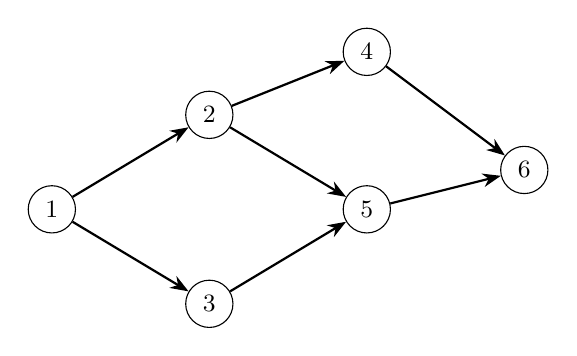
\begin{tikzpicture}[
        >=Stealth,
        v/.style={circle, draw, minimum size=6mm, font=\small},
        e/.style={->, thick},
        lbl/.style={font=\scriptsize, fill=white, inner sep=1pt}
    ]
        \node[v] (v1) at (0,0)   {1};
        \node[v] (v2) at (2,1.2) {2};
        \node[v] (v3) at (2,-1.2){3};
        \node[v] (v4) at (4,2.0) {4};
        \node[v] (v5) at (4,0)   {5};
        \node[v] (v6) at (6,0.5) {6};

        \draw[e] (v1) -- (v2);
        \draw[e] (v1) -- (v3);
        \draw[e] (v2) -- (v4);
        \draw[e] (v2) -- (v5);
        \draw[e] (v3) -- (v5);
        \draw[e] (v4) -- (v6);
        \draw[e] (v5) -- (v6);
    \end{tikzpicture}
    \caption{拓扑排序示例 AOV 网}
\end{figure}

\noindent 各顶点入度如下(统计每个顶点被指向的次数):
\[
indegree[1]=0,\ indegree[2]=1,\ indegree[3]=1,\ indegree[4]=1,\ indegree[5]=2,\ indegree[6]=2.
\]

\paragraph{步骤 1:初始化}
\[
S=\emptyset,\quad count=0.
\]

\paragraph{步骤 2:将入度为 0 的顶点压栈}
只有顶点 1 的入度为 0:
\[
S=\{1\}.
\]

\paragraph{步骤 3:循环出栈并更新入度}

\textbf{第 1 次循环:}
\begin{itemize}
    \item 弹栈:$v_j=1$,输出 1,$count=1$;
    \item 顶点 1 的邻接点是 2、3:
    \[
        indegree[2]:1\to 0,\quad indegree[3]:1\to 0.
    \]
    \item 入度变为 0 的顶点 2、3 入栈,例如先压 2 再压 3:
    \[
        S=\{2,3\}.
    \]
\end{itemize}

\textbf{第 2 次循环:}
\begin{itemize}
    \item 弹栈:$v_j=3$,输出 3,$count=2$;
    \item 顶点 3 的邻接点是 5:
    \[
        indegree[5]:2\to 1.
    \]
    \item 没有新的入度为 0 的顶点,栈中仍有:
    \[
        S=\{2\}.
    \]
\end{itemize}

\textbf{第 3 次循环:}
\begin{itemize}
    \item 弹栈:$v_j=2$,输出 2,$count=3$;
    \item 顶点 2 的邻接点是 4、5:
    \[
        indegree[4]:1\to 0,\quad indegree[5]:1\to 0.
    \]
    \item 顶点 4、5 入栈(例如先压 4 再压 5):
    \[
        S=\{4,5\}.
    \]
\end{itemize}

\textbf{第 4 次循环:}
\begin{itemize}
    \item 弹栈:$v_j=5$,输出 5,$count=4$;
    \item 顶点 5 的邻接点是 6:
    \[
        indegree[6]:2\to 1.
    \]
    \item 没有新的入度为 0 的顶点:
    \[
        S=\{4\}.
    \]
\end{itemize}

\textbf{第 5 次循环:}
\begin{itemize}
    \item 弹栈:$v_j=4$,输出 4,$count=5$;
    \item 顶点 4 的邻接点是 6:
    \[
        indegree[6]:1\to 0.
    \]
    \item 顶点 6 入栈:
    \[
        S=\{6\}.
    \]
\end{itemize}

\textbf{第 6 次循环:}
\begin{itemize}
    \item 弹栈:$v_j=6$,输出 6,$count=6$;
    \item 顶点 6 没有后继,入度数组不再变化,栈变空:
    \[
        S=\emptyset.
    \]
\end{itemize}

\paragraph{步骤 4:判断是否有回路}
此时
\[
count=6 = vertexNum,
\]
说明所有顶点都被输出,图中不存在回路,输出序列
\[
1,\ 3,\ 2,\ 5,\ 4,\ 6
\]
就是图 $G$ 的一个拓扑序列。\\

\noindent 若某个有向图中存在回路,则在某一步之后栈 $S$ 会变空,但仍有顶点入度 $>0$,此时 $count<vertexNum$,根据步骤 4 可判断图中存在有向回路。

\subsection{AOE网}
\subsubsection{基本概念}
\indent \pmb{AOE网(Activity on Edge Network)}:在一个表示工程的带权有向图中,用顶点表示\pmb{事件},用有向边表示\pmb{活动},边上的权值表示活动的\pmb{持续时间},
称这样的有向图叫做边表示的网,简称AOE网。
\indent AOE网中没有入边的顶点称为始点(或源点),没有出边的顶点称为终点(或汇点)。
\indent 只有在某顶点所代表的事件发生后,从该顶点出发的各活动才能开始。只有在进入某顶点的各活动都结束,该顶点所代表的事件才能发生。

\subsection{关键路径问题}
\subsubsection{基本概念}
\begin{enumerate}
    \item 关键路径:在AOE网中,从始点到终点具有最大路径长度(该路径上的各个活动所持续的时间之和)的路径称为关键路径。
    \item 关键活动:关键路径上的各活动称为关键活动。
\end{enumerate}
\indent 要找出关键路径,必须找出关键活动。

\subsubsection{算法步骤}
\indent 首先计算:
\begin{enumerate}
    \item 事件的最早发生时间ve[k]
    \item 事件的最晚发生时间vl[k]
    \item 活动的最早开始时间e[i]
    \item 活动的最晚开始时间l[i]
\end{enumerate}
对任意一个活动,如果满足:
\[
    l[i] - e[i] = 0
\]
则它无法“休息”,是关键活动。

\paragraph{计算ve[k]}
ve[k]是指从始点开始到顶点$v_k$的最大路径长度。
这个长度决定了所有从顶点$v_k$发出的活动能够开工的最早时间。即:

\[
    ve[0] = 0,
\]
\[
    ve[k] = \max_{\, (i,k)\in E}\{\, ve[i] + w(i,k) \},\quad k = 1,2,\dots,n-1,
\]

其中 $(i,k)\in E$ 表示从事件 $v_i$ 到事件 $v_k$ 有一条活动弧,$w(i,k)$ 为该活动的持续时间。\\
事实上,这里计算顺序是按照拓扑顺序。

\paragraph{计算vl[k]}
vl[k]是指在不推迟整个工期的前提下,事件vk允许的最晚发生时间。

\[
    vl[n-1] = ve[n-1],
\]
\[
    vl[k] = \min_{\, (k,j)\in E}\{\, vl[j] - w(k,j) \},\quad k = n-2,n-3,\dots,0,
\]
其中 $(k,j)\in E$ 表示从事件 $v_k$ 到事件 $v_j$ 有一条活动弧,$w(k,j)$ 为该活动的持续时间。\\
事实上,这里计算顺序是按照逆拓扑顺序。

\paragraph{计算e[i]}
若活动$a_i$是由弧$<v_k , v_j>$表示,则活动$a_i$的最早开始时间应等于事件$v_k$的最早发生时间。
\[
    e[i] = ve[k]
\]

\paragraph{计算l[i]}
若活动$a_i$是由弧$<v_k , v_j>$表示,则活动$a_i$的最晚开始时间要保证事件$v_j$的最迟发生时间不拖后。
\[
    l[i] = vl[j] - w(k,j) 
\]



\subsubsection{举例分析}
\indent 构造一个 AOE 网 $G=(V,E)$,顶点表示事件,边表示活动,边权为持续时间。\\
事件集合:
\[
V=\{v_0,v_1,v_2,v_3,v_4,v_5\},
\]
活动及持续时间(有向弧):
\[
\begin{aligned}
&a_1:(v_0,v_1,3),\quad a_2:(v_0,v_2,2),\quad a_3:(v_1,v_3,2),\\
&a_4:(v_2,v_3,4),\quad a_5:(v_1,v_4,4),\quad a_6:(v_3,v_5,3),\quad a_7:(v_4,v_5,2).
\end{aligned}
\]

\begin{figure}[h]
    \centering
    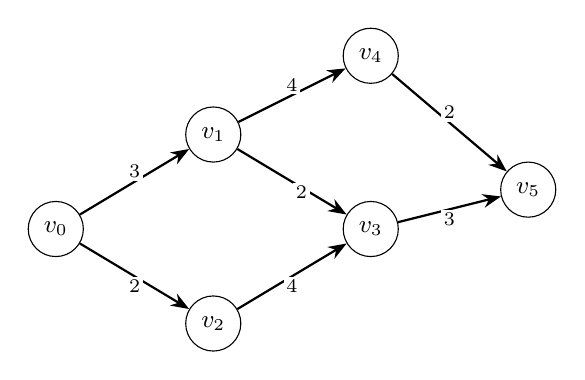
\begin{tikzpicture}[
        >=Stealth,
        v/.style={circle, draw, minimum size=7mm, font=\small},
        e/.style={->, thick},
        w/.style={font=\scriptsize, fill=white, inner sep=1pt}
    ]
        \node[v] (v0) at (0,0)   {$v_0$};
        \node[v] (v1) at (2,1.2) {$v_1$};
        \node[v] (v2) at (2,-1.2){$v_2$};
        \node[v] (v3) at (4,0)   {$v_3$};
        \node[v] (v4) at (4,2.2) {$v_4$};
        \node[v] (v5) at (6,0.5) {$v_5$};

        \draw[e] (v0) -- (v1) node[midway, above,  w]{$3$};
        \draw[e] (v0) -- (v2) node[midway, below,  w]{$2$};
        \draw[e] (v1) -- (v3) node[midway, below right, w]{$2$};
        \draw[e] (v2) -- (v3) node[midway, below,  w]{$4$};
        \draw[e] (v1) -- (v4) node[midway, above,  w]{$4$};
        \draw[e] (v3) -- (v5) node[midway, below,  w]{$3$};
        \draw[e] (v4) -- (v5) node[midway, above,  w]{$2$};
    \end{tikzpicture}
    \caption{AOE 网示例及持续时间}
\end{figure}

\paragraph{1. 拓扑排序}
该 AOE 网是一个 DAG,按照入度为 0 开始拓扑排序,可得到一个拓扑序列:
\[
v_0,\ v_1,\ v_2,\ v_4,\ v_3,\ v_5.
\]
(只要满足拓扑关系即可,具体顺序可能有多种,这里取其中一种。)

\paragraph{2. 计算事件的最早发生时间 ve[k]}
按拓扑序从前往后计算,令始点 $v_0$ 为 0:
\[
ve[0]=0.
\]
\[
\begin{aligned}
ve[1]&=\max\{ve[0]+w(0,1)\}=\max\{0+3\}=3;\\[2pt]
ve[2]&=\max\{ve[0]+w(0,2)\}=\max\{0+2\}=2;\\[2pt]
ve[4]&=\max\{ve[1]+w(1,4)\}=\max\{3+4\}=7;\\[2pt]
ve[3]&=\max\{ve[1]+w(1,3),\ ve[2]+w(2,3)\}\\
     &=\max\{3+2,\ 2+4\}=\max\{5,6\}=6;\\[2pt]
ve[5]&=\max\{ve[3]+w(3,5),\ ve[4]+w(4,5)\}\\
     &=\max\{6+3,\ 7+2\}=\max\{9,9\}=9.
\end{aligned}
\]

\noindent 整体结果:
\[
ve[0]=0,\ ve[1]=3,\ ve[2]=2,\ ve[3]=6,\ ve[4]=7,\ ve[5]=9.
\]

\paragraph{3. 计算事件的最晚发生时间 vl[k]}
令终点 $v_5$ 的最晚发生时间等于工程总工期:
\[
vl[5]=ve[5]=9.
\]
按\pmb{逆拓扑序}从后往前计算:
\[
v_5,\ v_3,\ v_4,\ v_2,\ v_1,\ v_0.
\]
\[
\begin{aligned}
vl[3]&=\min\{vl[5]-w(3,5)\}=\min\{9-3\}=6;\\[2pt]
vl[4]&=\min\{vl[5]-w(4,5)\}=\min\{9-2\}=7;\\[2pt]
vl[2]&=\min\{vl[3]-w(2,3)\}=\min\{6-4\}=2;\\[2pt]
vl[1]&=\min\{vl[3]-w(1,3),\ vl[4]-w(1,4)\}\\
     &=\min\{6-2,\ 7-4\}=\min\{4,3\}=3;\\[2pt]
vl[0]&=\min\{vl[1]-w(0,1),\ vl[2]-w(0,2)\}\\
     &=\min\{3-3,\ 2-2\}=\min\{0,0\}=0.
\end{aligned}
\]

\noindent 整体结果:
\[
vl[0]=0,\ vl[1]=3,\ vl[2]=2,\ vl[3]=6,\ vl[4]=7,\ vl[5]=9.
\]

\paragraph{4. 计算活动的 e[i]、l[i] 并找关键活动}
对每条活动弧 $a_i:\langle v_k,v_j\rangle$:
\[
e[i]=ve[k],\qquad l[i]=vl[j]-w(k,j).
\]

\[
\begin{array}{c|c|c|c|c}
\hline
\text{活动} & \text{弧} & e[i] & l[i] & l[i]-e[i]\\
\hline
a_1 & (v_0,v_1,3) & ve[0]=0 & vl[1]-3=3-3=0 & 0\\
a_2 & (v_0,v_2,2) & ve[0]=0 & vl[2]-2=2-2=0 & 0\\
a_3 & (v_1,v_3,2) & ve[1]=3 & vl[3]-2=6-2=4 & 1\\
a_4 & (v_2,v_3,4) & ve[2]=2 & vl[3]-4=6-4=2 & 0\\
a_5 & (v_1,v_4,4) & ve[1]=3 & vl[4]-4=7-4=3 & 0\\
a_6 & (v_3,v_5,3) & ve[3]=6 & vl[5]-3=9-3=6 & 0\\
a_7 & (v_4,v_5,2) & ve[4]=7 & vl[5]-2=9-2=7 & 0\\
\hline
\end{array}
\]

\noindent 对满足
\[
l[i]-e[i]=0
\]
的活动,它们没有机动时间,属于\pmb{关键活动}。由上表可见:
\[
a_1,\ a_2,\ a_4,\ a_5,\ a_6,\ a_7
\]
都是关键活动。其中一条关键路径例如:
\[
v_0 \xrightarrow{a_1} v_1 \xrightarrow{a_5} v_4 \xrightarrow{a_7} v_5,
\]
其总时间为 $3+4+2=9$;另一条关键路径为
\[
v_0 \xrightarrow{a_2} v_2 \xrightarrow{a_4} v_3 \xrightarrow{a_6} v_5,
\]
其总时间同样为 $2+4+3=9$。这两条路径的长度都等于 $ve[5]$,因此都是关键路径。



\end{document}